\documentclass[pdf,aspectratio=169]{beamer}

\usepackage[utf8]{inputenc}
\usepackage[vietnamese]{babel}
\usepackage{microtype}
\usepackage{lmodern}
\usepackage{breqn}
\usepackage{nicefrac}
\usepackage{amsmath,amsthm,amssymb}
\usepackage{mathtools}
\usepackage{grffile}
\usepackage{physics}
\usepackage{graphicx}
\usepackage{lipsum}  
\usepackage{tikz} % Package for drawing
\usepackage{hyperref}
\usepackage{pgfplots}
\usetikzlibrary{snakes,arrows,shapes}
\usetikzlibrary{plotmarks}
\usetikzlibrary{arrows.meta}
\usepgfplotslibrary{patchplots}
\DeclareUnicodeCharacter{2212}{−}
\usepgfplotslibrary{groupplots,dateplot}
\usetikzlibrary{patterns,shapes.arrows}
\pgfplotsset{compat=newest}
\DeclarePairedDelimiter\ceil{\lceil}{\rceil}
\DeclarePairedDelimiter\floor{\lfloor}{\rfloor}

% command for common set
\newcommand{\N}{\mathbb{N}}
\newcommand{\Z}{\mathbb{Z}}
\newcommand{\R}{\mathbb{R}}
\newcommand{\C}{\mathbb{C}}

%theorems
\newtheorem{question}{Question}
\newtheorem*{vidu}{Ví dụ}
%theme settings
\usetheme{Madrid}
\usecolortheme{default}
\definecolor{cam}{rgb}{0.9686,0.4039,0.1529} %247, 103, 39
%\definecolor{xanh}{rgb}{0.2314, 0.7412, 0.7922} %59, 189, 202
\definecolor{xanh}{rgb}{0.2235, 0.6980, 0.7412} %57, 178, 189
\setbeamercolor*{palette primary}{bg=xanh, fg=white}
\setbeamercolor*{palette secondary}{bg=white, fg=cam}
\setbeamercolor*{palette tertiary}{bg=white, fg=black}
\setbeamercolor*{palette quaternary}{bg=xanh, fg=white}
\beamertemplatenavigationsymbolsempty
\AtBeginEnvironment{question}{%
    \setbeamercolor{block body}{bg=white, fg=black}
    \setbeamercolor{block title}{bg=cam, fg=white}
    }
\AtBeginEnvironment{theorem}{%
    \setbeamercolor{block body}{bg=white, fg=black}
    \setbeamercolor{block title}{bg=cam, fg=white}
    }
\AtBeginEnvironment{lemma}{%
    \setbeamercolor{block body}{bg=white, fg=black}
    \setbeamercolor{block title}{bg=cam, fg=white}
    }
\AtBeginEnvironment{problem}{%
    \setbeamercolor{block body}{bg=white, fg=black}
    \setbeamercolor{block title}{bg=cam, fg=white}
    }
\AtBeginEnvironment{solution}{%
    \setbeamercolor{block body}{bg=white, fg=black}
    \setbeamercolor{block title}{bg=cam, fg=white}
    }
\AtBeginEnvironment{proof}{%
    \setbeamercolor{block body}{bg=white, fg=black}
    \setbeamercolor{block title}{bg=cam, fg=white}
    }
\AtBeginEnvironment{vidu}{%
    \setbeamercolor{block body}{bg=white, fg=black}
    \setbeamercolor{block title}{bg=cam, fg=white}
    }


\titlegraphic{\vspace{1cm}
\includegraphics[width=2cm]{figs/logo.png}}
% add logo
\addtobeamertemplate{frametitle}{}{%
    \begin{tikzpicture}[remember picture,overlay]
        \fill[xanh] (13.6,0.6) circle (.9cm);
        \clip (13.6,0.6) circle (.75cm);
        \node at (13.6,0.6) {
\includegraphics[width=1.3cm]{figs/white_logo.png}};
    \end{tikzpicture}
    }


%Hyperref setup
\hypersetup{colorlinks,citecolor=blue,filecolor=blue,linkcolor=blue,urlcolor=blue}

\mode<presentation>{}

\title{\textbf{Math Biology Cơ bản}}
\subtitle{Mô hình hóa Toán học và ứng dụng trong Sinh học}
\author{Nguyễn Trần Nam Tiến}
\date{}
\bibliographystyle{abbrv}

\begin{document}

\begin{frame}
    \titlepage
\end{frame}

\begin{frame}[plain]
    \begin{center}
        \vspace{1cm}
        \Huge Giới thiệu về mô hình hóa
    \end{center}
\end{frame}

%===============
\begin{frame}{Mô hình hóa là gì?}
    Mô hình hóa toán học là quá trình chuyển đổi các vấn đề thực tế thành dạng ký hiệu để phân tích và giải quyết các vấn đề đó.
    Mô hình hóa toán học có thể được biểu diễn bằng đồ thị sau:
    \begin{center}
        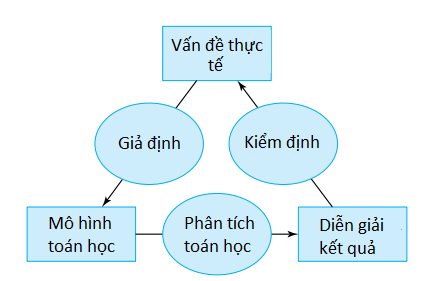
\includegraphics[width=5cm]{figs/math_model.png}
    \end{center}
    \begin{itemize}
        \item Xây dựng mô hình toán học bằng cách công thức hóa các vấn đề thực tế
        \item Phân tích và tìm ra lời giải cho bài toán
        \item Diễn giải kết quả của bài toán cho phù hợp với với đề thực tế
    \end{itemize}
\end{frame}

\begin{frame}{Các dạng mô hình hóa}
    Có rất nhiều điều kiện để phân loại các dạng mô hình hóa toán học. Có thể kể đến như sau
    \begin{enumerate}
        \item \textbf{Linear vs Nonlinear}: mô hình có các toán tử là tuyến tính hay phi tuyến
        \item \textbf{Static vs Dynamic}: mô hình có phụ thuộc vào thời gian hay ko
        \item \textbf{Discrete vs Continuous}: mô hình coi vấn đề thực tế liên tục hay rời rạc
        \item \textbf{Deterministic vs Probabilistic}: mô hình có các yếu tố ngẫu nhiên hay không 
    \end{enumerate}
\end{frame}

\begin{frame}[plain]
    \begin{center}
        \vspace{1cm}
        \Huge Mô hình hóa toán học và Toán sinh học
    \end{center}
\end{frame}

\begin{frame}{Mô hình hóa toán học và Toán sinh học}
    \textbf{Toán sinh học (hay Sinh học lý thuyết)}, là một nhánh của Sinh học
    sử dụng các phân tích lý thuyết, mô hình toán học và trừu tượng hóa các sinh vật sống
    để nghiên cứu các nguyên lý đại diện cho cấu trúc, sự phát triển và hành vi của các hệ sinh học. \\
    Các dạng mô hình hóa trong Toán sinh học cũng tương tự như slide trước. Tuy nhiên, trong phạm vi
    phần đầu khóa học này chúng ta tập trung vào \textbf{\textit{phương trình sai phân}} - một \textbf{\textit{discrete dynamical system}} vì các lý do sau:
    \begin{enumerate}
        \item Modeling with difference equations is a very powerful, yet
              simple tool for modeling dynamical systems in biology, ecology,
              the environment, and chemistry
        \item Modeling with difference equations requires knowledge of
              algebra but does not require knowledge of differential calculus
        \item Đối tượng khóa học tập trung vào các bạn học sinh cấp 3 và năm nhất, năm hai đại học,
              chưa có kiến thức nhiều về các nhánh của toán học như Phương trinh vi phân, phương trình đạo hàm riêng, ...
    \end{enumerate}
\end{frame}

\begin{frame}{Mô hình hóa toán học và Toán sinh học}
    \begin{vidu}
        Consider the population of a city with a constant growth rate per year. The
        population is counted at the end of each year. For simplicity, assume that
        there is no immigration to or emigration from the city.\\
        i. Model the population dynamic and predict the long-term behavior
        of the system.\\
        ii. In 2020, the city’s population was 100,000. The natural annual
        growth rate of the population is 1\% per year. Predict the city’s
        population in 2030. Estimate the population over the next 30 years
        and graph it. What is the long-term behavior of the population?
    \end{vidu}
\end{frame}

\begin{frame}{Mô hình hóa toán học và Toán sinh học}
    \textbf{Bàn Luận} \\
    i. We will measure the population at discrete time intervals in
    one-year units. Đặt: \\
    \quad $p_n$ là dân số tại thời điểm kết thúc năm thứ $n$ \\
    \quad $p_0$ là dân số ban đầu \\
    \quad $r$ là tốc độ gia tăng dân số \\
    Ta có mối liên hệ giữa dân số năm thứ $n+1$ và năm thứ $n$:
    \begin{align}
        \label{eq:1}
        p_{n+1} = p_n + rp_n = (1+r)p_n
    \end{align}
    Phương trình \ref{eq:1} là một \textit{phương trình sai phân} (hay phương trình đệ quy).
    Phương trình này kết hợp với điều kiện dân số ban đầu $p_0$ đại diện cho sự thay đổi động lực học của dân số.
    Bởi vì dân số thay đổi theo thời gian, nên đây là một \textbf{\textit{dynamical system}}.
    Chúng ta cũng mô phỏng hệ theo các khoảng thời gian rời rạc, nên đây là một \textbf{\textit{discrete system}}.
    Như vậy, bài toán thực tế về dân số đã được \textbf{\textit{mô hình hóa}} bằng một \textbf{\textit{discrete dynamical system}}.
\end{frame}

\begin{frame}{Mô hình hóa toán học và Toán sinh học}
    \textbf{Bàn Luận (tiếp):} \\
    Để giải hệ trên, giả sử để tìm $p_k$ ta có thể thay $p_0$ vào phương trình \ref{eq:1} để tìm $p_1$, rồi tìm $p_2$,
    lần lượt đến $p_k$. Bằng phương pháp trên, với mọi $k$ ta luôn tìm được một dãy số: \\
    \quad $p_0, p_1, p_2, ..., p_k$\\
    là nghiệm của phương trình \ref{eq:1}. Đây được gọi là \textbf{\textit{nghiệm số học (numerical solution)}} của phương trình mô hình hóa.\\
    Ta cũng có thể dễ dàng chứng minh được từ phương trình \ref{eq:1}
    \begin{align}
        \label{eq:2}
        p_{n} = (1+r)^np_0
    \end{align}
    với $n\in \N$. Đây được gọi là \textbf{\textit{nghiệm chính xác (exact solution hay analytical solution)}} của phương trình mô hình hóa.\\
    Phương trình \ref{eq:2} là một hàm số mũ. Nếu $r>0$, $1+r>1$ thì $p_{n}$ sẽ tiến tới vô cùng.
    Nếu $r<0$, $1+r<1$ thì $p_{n}$ sẽ tiến tới $0$ khi $n$ tiến tới vô cùng. (Đây là bước biện giải mô hình hóa toán học)
\end{frame}

\begin{frame}{Mô hình hóa toán học và Toán sinh học}
    \textbf{Bàn Luận (tiếp):} \\
    ii. Ta có $n=10, p_0 = 100000, r=0.01$. Tại năm thứ $10$, dân số của thành phố là:
    $$p_{10}=(1+0.01)^{10}100000=110462$$
    Để vẽ đồ thị, ta tính dãy số $p_0, p_1, p_2,...,p_{30}$ theo phương trình \ref{eq:2}. Kết quả như sau:
    \begin{center}
        \begin{tikzpicture}[scale=0.5]

            \definecolor{color0}{rgb}{0.12156862745098,0.466666666666667,0.705882352941177}

            \begin{axis}[
                    tick align=outside,
                    tick pos=left,
                    x grid style={white!69.0196078431373!black},
                    xlabel={Thời gian năm thứ $n$},
                    xmin=-1.5, xmax=31.5,
                    xtick style={color=black},
                    y grid style={white!69.0196078431373!black},
                    ylabel={Dân số $p_n$},
                    ymin=98260.8, ymax=136523.2,
                    ytick style={color=black}
                ]
                \addplot [semithick, color0, mark=*, mark size=2, mark options={solid}, only marks]
                table[row sep=\\] {%
                        0 100000\\
                        1 101000\\
                        2 102010\\
                        3 103030\\
                        4 104060\\
                        5 105101\\
                        6 106152\\
                        7 107213\\
                        8 108285\\
                        9 109368\\
                        10 110462\\
                        11 111566\\
                        12 112682\\
                        13 113809\\
                        14 114947\\
                        15 116096\\
                        16 117257\\
                        17 118430\\
                        18 119614\\
                        19 120810\\
                        20 122019\\
                        21 123239\\
                        22 124471\\
                        23 125716\\
                        24 126973\\
                        25 128243\\
                        26 129525\\
                        27 130820\\
                        28 132129\\
                        29 133450\\
                        30 134784\\
                    };
            \end{axis}

        \end{tikzpicture}
    \end{center}

\end{frame}

\begin{frame}{Mục tiêu khóa học}
    \begin{itemize}
        \item Hiểu và nắm được bản chất của mô hình hóa toán học
        \item Ứng dụng mô hình hóa toán học vào sinh học
        \item Sử dụng các công cụ toán học và tin học trong mô hình hóa toán học
    \end{itemize}
\end{frame}

%===============
%\begin{frame}
%    \frametitle{References}
%    \bibliography{bib}
%\end{frame}

%===============

\begin{frame}[plain]
    \begin{center}
        \vspace{1cm}
        \Huge THANK YOU!
    \end{center}
\end{frame}

\end{document}